\subsection{积与纤维积}

命题 2. --- 设 B 与 B' 为拓扑空间，(E, p) 为 B-空间，(E', p') 为 B'-空间。假设 E 与 E' 是局部平凡纤维空间（相应地，覆叠）。则空间 E × E' 赋有映射 p × p': E × E' → B × B' 后，是以 B × B' 为基的局部平凡纤维空间（相应地，覆叠）。若 E 与 E' 是可平凡化的，则 E × E' 亦然。

首先假设 B-空间 E 与 B'-空间 E' 分别有平凡化 \(g: E \to B \times F\) 与 \(g': E' \to B' \times F'\)。把同胚 \(g \times g'\) （从 \(E \times E'\) 到 \((B \times F) \times (B' \times F')\) 上的）与从 \((B \times F) \times (B' \times F')\) 到 \((B \times B') \times (F \times F')\) 上的典范同胚复合，便得到 \(B \times B'\)-空间 \(E \times E'\) 的一个以 \(F \times F'\) 为纤维型的平凡化。若 F 与 \(F'\) 是离散空间，则空间 \(F \times F'\) 也是离散的。

在一般情形，对任一点 \((a, a')\) （\(B \times B'\) 的），存在 a 在 B 中的邻域 U 与邻域 \(U'\) （\(a'\) 在 B' 中的），使得 U-空间 \(E_{U}\) 与 \(U'\)-空间 \(E_{U'}\) 都是可平凡化的。由前所证，\(B \times B'\)-空间 \(E \times E'\) 在 \(U \times U'\) 上是可平凡化的。因而它是以 \(B \times B'\) 为基的局部平凡纤维空间。若 E 与 \(E'\) 是覆叠，则其诸纤维是离散的，由此即得命题。

注意，若 \((p_{i} \colon \mathrm{E}_{i} \to \mathrm{B}_{i})_{i \in \mathrm{I}}\) 是局部平凡纤维空间的一族，甚至是覆叠的一族，则积空间 \(\prod_{i \in I} E_{i}\) 赋以映射 \((p_{i})_{i \in I}\) 后，不一定是以 \(\prod_{i \in I} B_{i}\) 为基的局部平凡纤维空间 (I, p. 145, exerc. 3)。

推论 1. --- 设 A 为拓扑空间，并设 B、B' 为 A-空间。设 E 与 E' 是分别以 B 与 B' 为基的局部平凡纤维空间（相应地，覆叠）；用 p 与 p' 表示它们的投影。则由 p × p' 通过过渡到子空间而得的 \(B \times_{A} B'\)-空间 \(E \times_{A} E'\) 是局部平凡纤维空间（相应地，覆叠）。若 E 与 E' 是可平凡化的，则它亦然。

由于集合 \(E \times_{A} E'\) 是 \(B \times_{A} B'\) 在映射 \(p \times p'\) : \(E \times E' \to B \times B'\) 下的逆像，故推论由命题 2 及注 1 (I, p. 68) 得出。

推论 2. --- 设

\pandocbounded{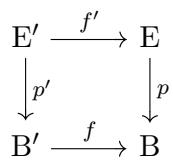
\includegraphics[keepaspectratio]{images/part001_3dd3ce93.jpg}}

一个笛卡尔方块。若 (E,p) 是局部平凡 B-纤维空间（相应地，覆叠），则 (E',p') 是以 B' 为基的局部平凡纤维空间（相应地，覆叠），且当 (E,p) 可平凡化时它亦可平凡化。

这由推论 1 得出，取其中 B = A 且 E' = B'。

推论 3. --- 设 B 为拓扑空间。设 E 与 E' 是局部平凡 B-纤维空间（相应地，覆叠）。则 \(E \times_{B} E'\) 是局部平凡 B-纤维空间（相应地，B 的覆叠）。若 E 与 E' 是可平凡化的，则它亦然。

这由推论 1 得出，取 A、B、B' 相等的情形。

命题 3. --- 设

\begin{enumerate}
\def\labelenumi{(\arabic{enumi})}
\tightlist
\item
\end{enumerate}

\pandocbounded{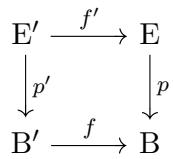
\includegraphics[keepaspectratio]{images/part001_0991252f.jpg}}

一个笛卡尔方块。假设在 B 的每一点的一个邻域内，映射 f 都有连续截面。那么，若 (E', p') 是局部平凡 B'-纤维空间（相应地，覆叠），则 B-空间 (E, p) 是局部平凡纤维空间（相应地，覆叠）。

须证 B 的每一点 \(a\) 都有邻域 U，使得 \((\mathrm{E}, p)\) 在 U 上诱导的 U-空间是局部平凡纤维空间（相应地，覆叠）。取 \(a\) 的、在其上存在连续截面 \(s\) （\(f\) 的）的一个邻域作为 U。用 \(i: \mathrm{U} \to \mathrm{B}\) 与 \(j: \overline{p}^{-1}(\mathrm{U}) \to \mathrm{E}\) 表示典范单射。由于方块 (1) 是笛卡尔的，存在唯一的连续映射 \(s^{\prime}\colon \overline{p}^{1}(\mathrm{U})\to \mathrm{E}^{\prime}\) 使得 \(f^{\prime}\circ s^{\prime} = j\) 且 \(p^{\prime}\circ s^{\prime} = s\circ p_{\mathrm{U}}\)。方块

\[
\begin{array}{c} \stackrel {{- 1}} {{p}} (\mathrm{U}) \xrightarrow {s ^ {\prime}} \mathrm{E} ^ {\prime} \\ \Biggl \downarrow p _ {\mathrm{U}} \\ \mathrm{U} \xrightarrow {s} \mathrm{B} ^ {\prime} \end{array}\tag{2}
\]

于是它是交换的，并且它与方块 (1) 的复合正是那个笛卡尔方块。

\[
\begin{array}{c} \overline {{p}} ^ {1} (\mathrm{U}) \xrightarrow {j} \mathrm{E} \\ \Biggl \downarrow p _ {\mathrm{U}} \\ \mathrm{U} \xrightarrow {i} \mathrm{B}. \end{array}
\]

由 I, p. 15 的命题 7，方块 (2) 是笛卡尔的。推论 2 使我们得以得出结论。

注意. --- 若在命题 3 中把关于映射 f 的假设减弱为只设它是普遍严格且满的，并且 \(p'\) 是覆叠，则映射 p 是平展的 (I, p. 31, prop. 8) 且是分离的 (I, p. 27, prop. 4)，但 E 不一定是 B 的覆叠。例如，可以找到拓扑空间 B、B 的局部有限闭覆盖 \((\mathrm{A}_{i})_{i\in\mathrm{I}}\) 以及一个不是覆叠的 B-空间 \((\mathrm{E},p)\)，使得对每个 \(i\in I\)，由 \(A_{i}\) 诱导的空间 \(E_{A_{i}}\) 是 \(A_{i}\) 的覆叠 (I, p. 146, exerc. 5)。但关于一个充分条件，可参见 I, p. 77 的推论 4。

